\begin{question}
Using \texttt{pandas} import data stored in \href{https://github.com/matteosan1/finance_course/raw/master/input_files/stock_market.xlsx}{stock\_market.xlsx}. With the resulting dataframe:
\begin{itemize}
\tightlist
\item remove duplicates and missing data (how many rows are left ?);
\item find stocks with positive variation;
\item determine the five lowest price stocks.
\end{itemize}
\end{question}

\cprotEnv\begin{solution}
First load the excel file into a dataframe and look at data structure.

\begin{ipython}
import pandas as pd

df = pd.read_excel("stock_market.xlsx")
print (len(df))
print (df.head())
\end{ipython}
\begin{ioutput}
52
  ticker       Price  Volume     Delta    Delta%     Market Cap
0    APH   65.654160  1.5950 -0.078423 -0.001178   46649.495552
1    HRL   44.971874  3.3267 -1.120468 -0.024254   24457.936896
2    REG   49.253113  0.8656 -0.360996 -0.007412   11351.617536
3    BWA   43.179356  4.8792  1.734138  0.042629   10611.859456
4   INTU  410.860809  1.1647  8.171570  0.019976  115895.599104
\end{ioutput}
        
If we are not sure that data is \emph{clean} we should check for duplicates and \texttt{NaN} and take care of them. The \texttt{duplicated} method returns the status of each row (duplicate or not, True or False). If we would like just to see the duplicated entries we could combine the \texttt{duplicated} method with the selection syntax like this:

\begin{ipython}
print(df[df.duplicated() == True])
\end{ipython}
\begin{ioutput}
   ticker       Price   Volume     Delta    Delta%     Market Cap
39    WDC   67.300003   6.0131  1.090004  0.016624   13900.362752
49    HII  170.458679   0.4316 -0.926727 -0.005507    8680.606720
51   QCOM  139.125961  11.9372 -0.788132 -0.005541  149658.779648
\end{ioutput}
        
So it looks like we have three duplicates and we can remove them:

\begin{ipython}
print (f"Before duplicates removal: {len(df)}")
df.drop_duplicates(inplace=True)
print (f"After duplicates removal: {len(df)}")
\end{ipython}
\begin{ioutput}
Before duplicates removal: 52
After duplicates removal: 49
\end{ioutput}

Then we need to take care of the \texttt{NaN}, again if we want to check the rows with \texttt{NaN} we can select (here the syntax is a little bit more complicated since we need to use \texttt{any} to look for \texttt{NaN} in every column):

\begin{ipython}
print ()df[df.isna().any(axis=1)])
\end{ipython}
\begin{ioutput}
   ticker       Price  Volume     Delta    Delta%     Market Cap
36   ODFL  206.511932  0.3687       NaN -0.009519   35271.376896
41    AAP         NaN  1.5906  2.566040  0.017669    8747.030528
46    ABT  123.174004  3.1618 -0.203285       NaN  193658.322944
\end{ioutput}
        
Since we don't want to artificially modify our sample we just drop rows with \texttt{NaN}:

\begin{ipython}
print (f"Before NaN removal: {len(df)}")
df.dropna(inplace=True)
print (f"After NaN removal: {len(df)}")
\end{ipython}
\begin{ioutput}
Before NaN removal: 49
After NaN removal: 46
\end{ioutput}

The second point asks to determine the companies with a daily positive variation. Clearly we have to apply to the dataframe a selection on the "Delta" (or "Delta\%") column requiring positive values.

\begin{ipython}
pos_var = df.loc[df["Delta"] > 0, :]
print (len(pos_var))
print (pos_var.head())
\end{ipython}
\begin{ioutput}
25
   ticker       Price   Volume     Delta    Delta%     Market Cap
3     BWA   43.179356  4.87920  1.734138  0.042629   10611.859456
4    INTU  410.860809  1.16470  8.171570  0.019976  115895.599104
5     RJF   75.888489  0.91605  2.174728  0.029352   24506.064896
6     CSX   29.297924  9.96330  0.198599  0.006767   63387.660288
10   CTVA   44.009796  1.87760  0.890366  0.020509   45105.881088
\end{ioutput}
        
So in origin we had 46 stocks and 25 of them have a positive variation of its price.

The last question requires to print the five lowest price stocks. In this case it is enough to sort by price the dataframe (ascending) and then just select the first five entries.

\begin{ipython}
highest_price = df.sort_values(by=['Price'], ascending=True)[:5]
highest_price
\end{ipython}
\begin{ioutput}
   ticker      Price     Volume     Delta    Delta%     Market Cap
27     RF  18.772100   6.377100  0.618860  0.033742   21679.149056
28      T  19.063257  67.769867  0.109594  0.005903  142539.997184
7     NWS  22.469374   0.901300 -0.294357 -0.012766   11940.613120
13    HWM  28.521683   1.581600  0.099586  0.003536   16887.724032
6     CSX  29.297924   9.963300  0.198599  0.006767   63387.660288
\end{ioutput}
\end{solution}

\begin{question}
Given the discount factors in \href{https://raw.githubusercontent.com/matteosan1/finance_course/master/input_files/exercise_5.28.csv}{exercise\_5.28.csv} plot the resulting discount curve, possibly adding axis labels and legend.
\end{question}

\cprotEnv\begin{solution}
\begin{ipython}
import pandas as pf
from datetime import date
from matplotlib import pyplot as plt
import matplotlib.dates as mdates

df = pd.read_csv("exercise_5.28.csv")
print (df.head())
dfs = df['dfs']
pillars = [d.date() for d in pd.to_datetime(df['pillars'])]

plt.plot(pillars, dfs, marker="o", label="EUR6M d.f.")

plt.gca().xaxis.set_major_formatter(mdates.DateFormatter('%Y-%m-%d'))
# this one instead rotate labels to avoid superimposition
plt.xticks(rotation=45)
plt.xlabel("Pillar dates")
plt.ylabel("Discount Factors")
plt.grid(True)
plt.legend()
plt.show()
\end{ipython}

\begin{figure}[htb]
\begin{center}
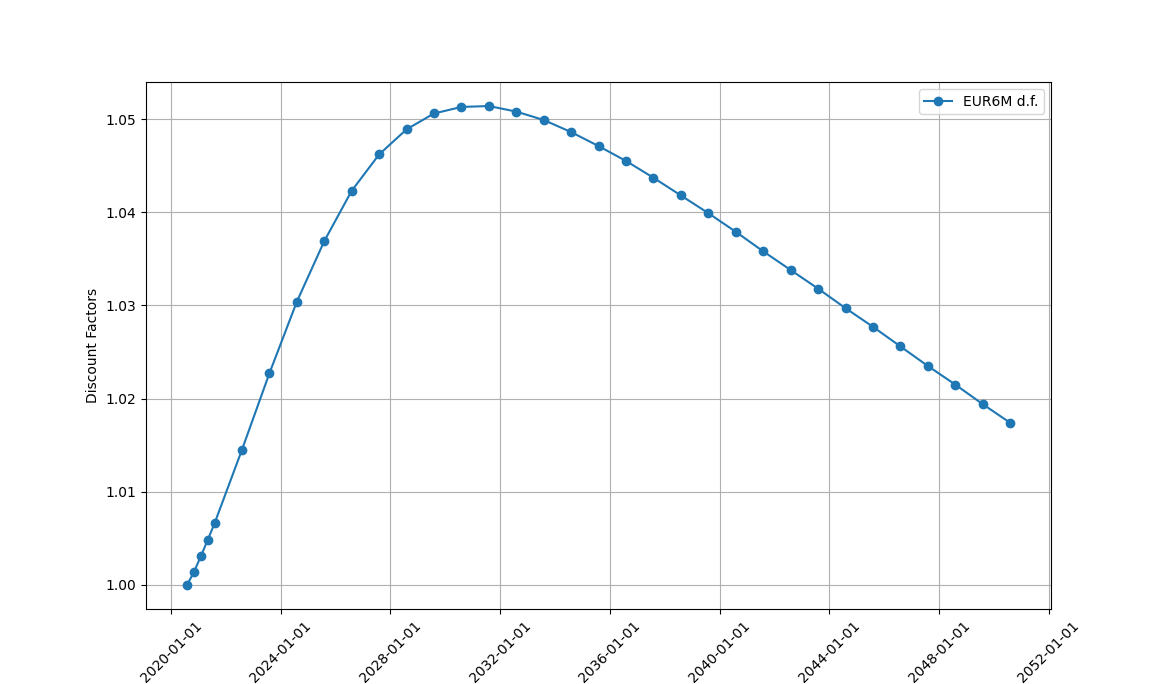
\includegraphics[width=0.7\linewidth]{figures/ex5.5}
\end{center}
\end{figure}
\end{solution}



